% Print results for comparing MSN with Heaviside jump function

\begin{figure}[p]
    \centering
    \begin{subfigure}{0.45\textwidth}
    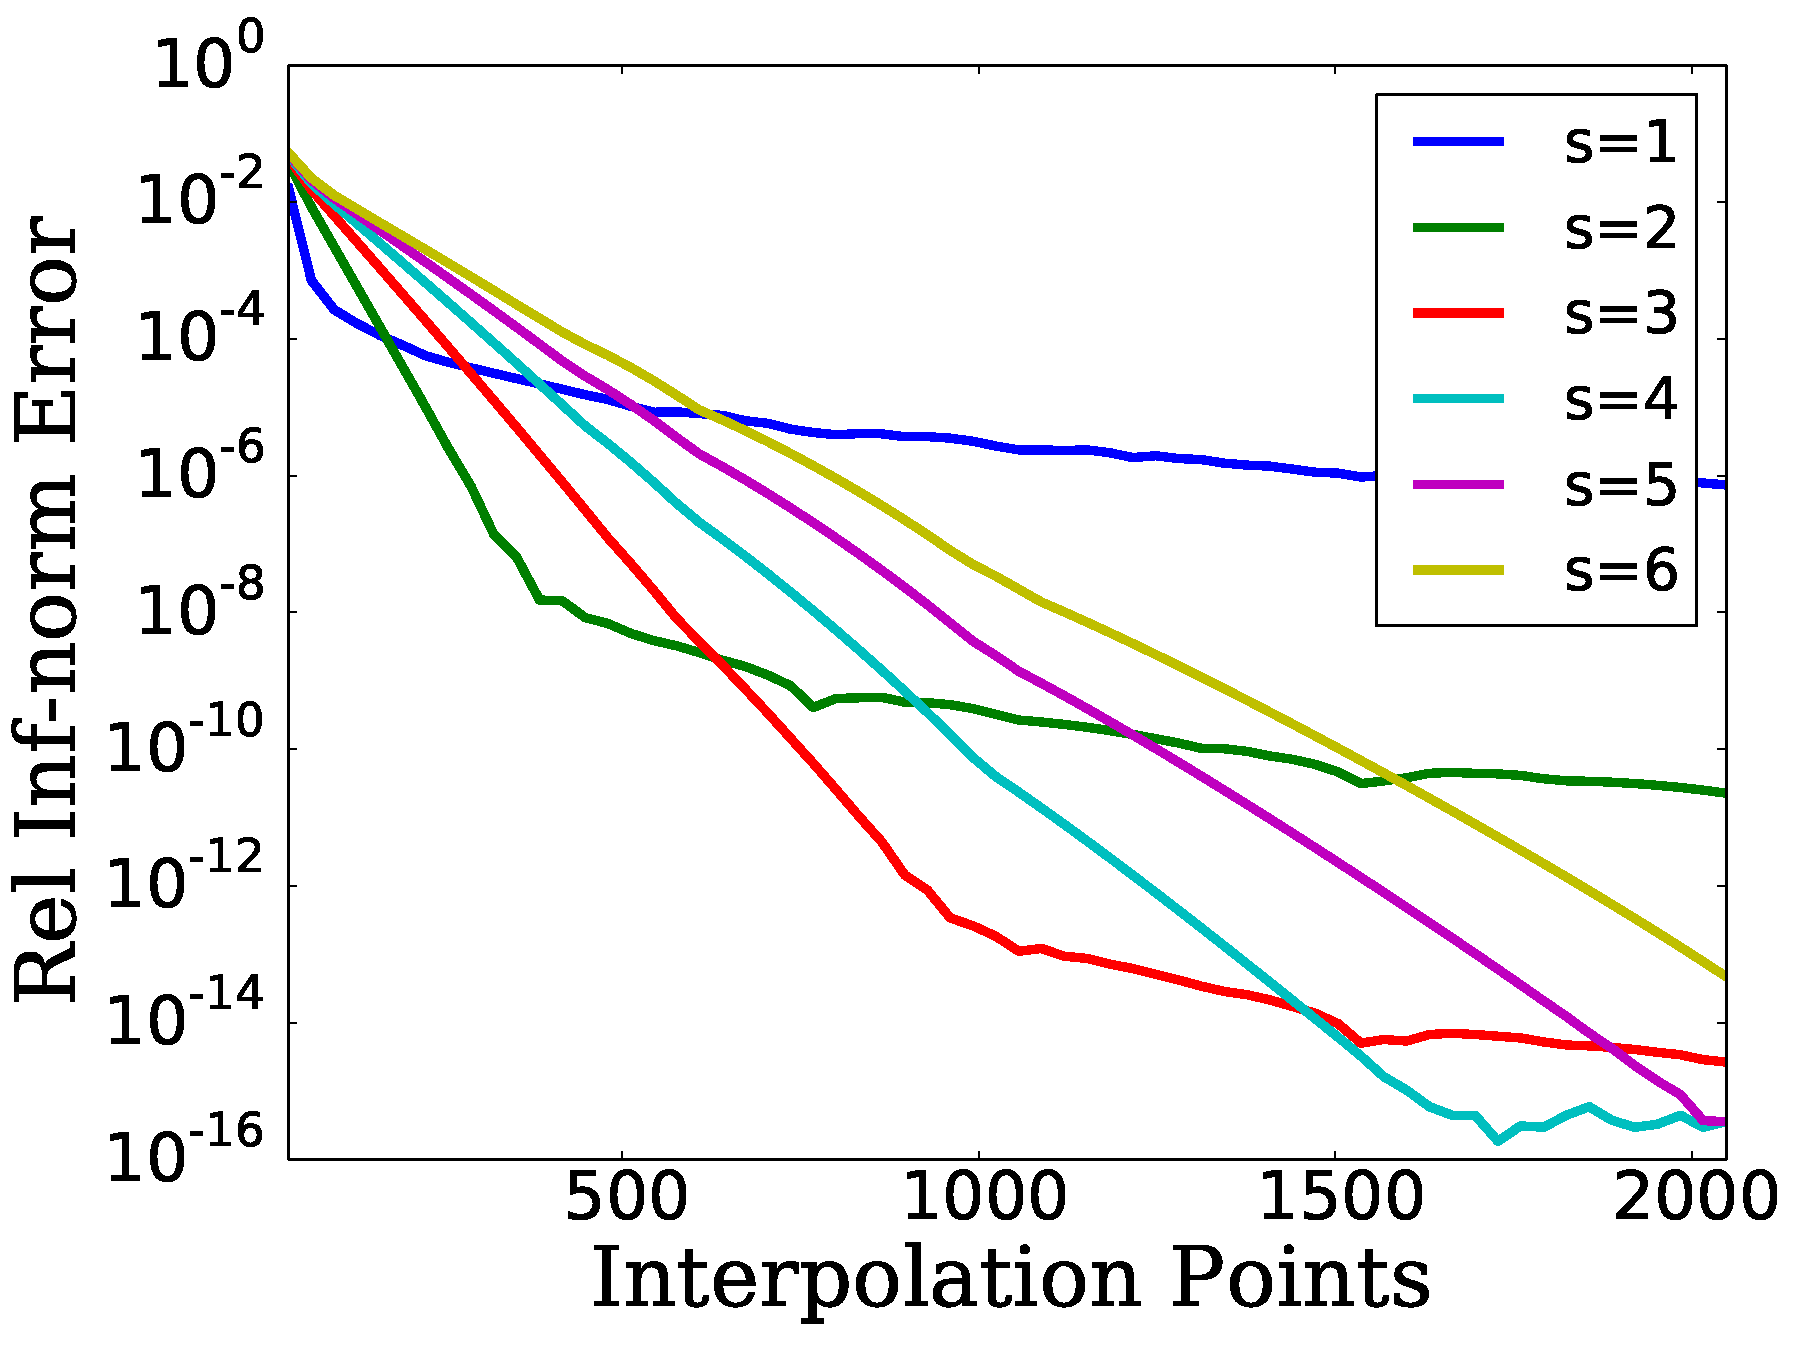
\includegraphics[width=\textwidth]{plots/msn_interp_fast_2n_rough_heaviside_2.pdf}
    \caption{Degree $2n$}
    \end{subfigure}
    \begin{subfigure}{0.45\textwidth}
    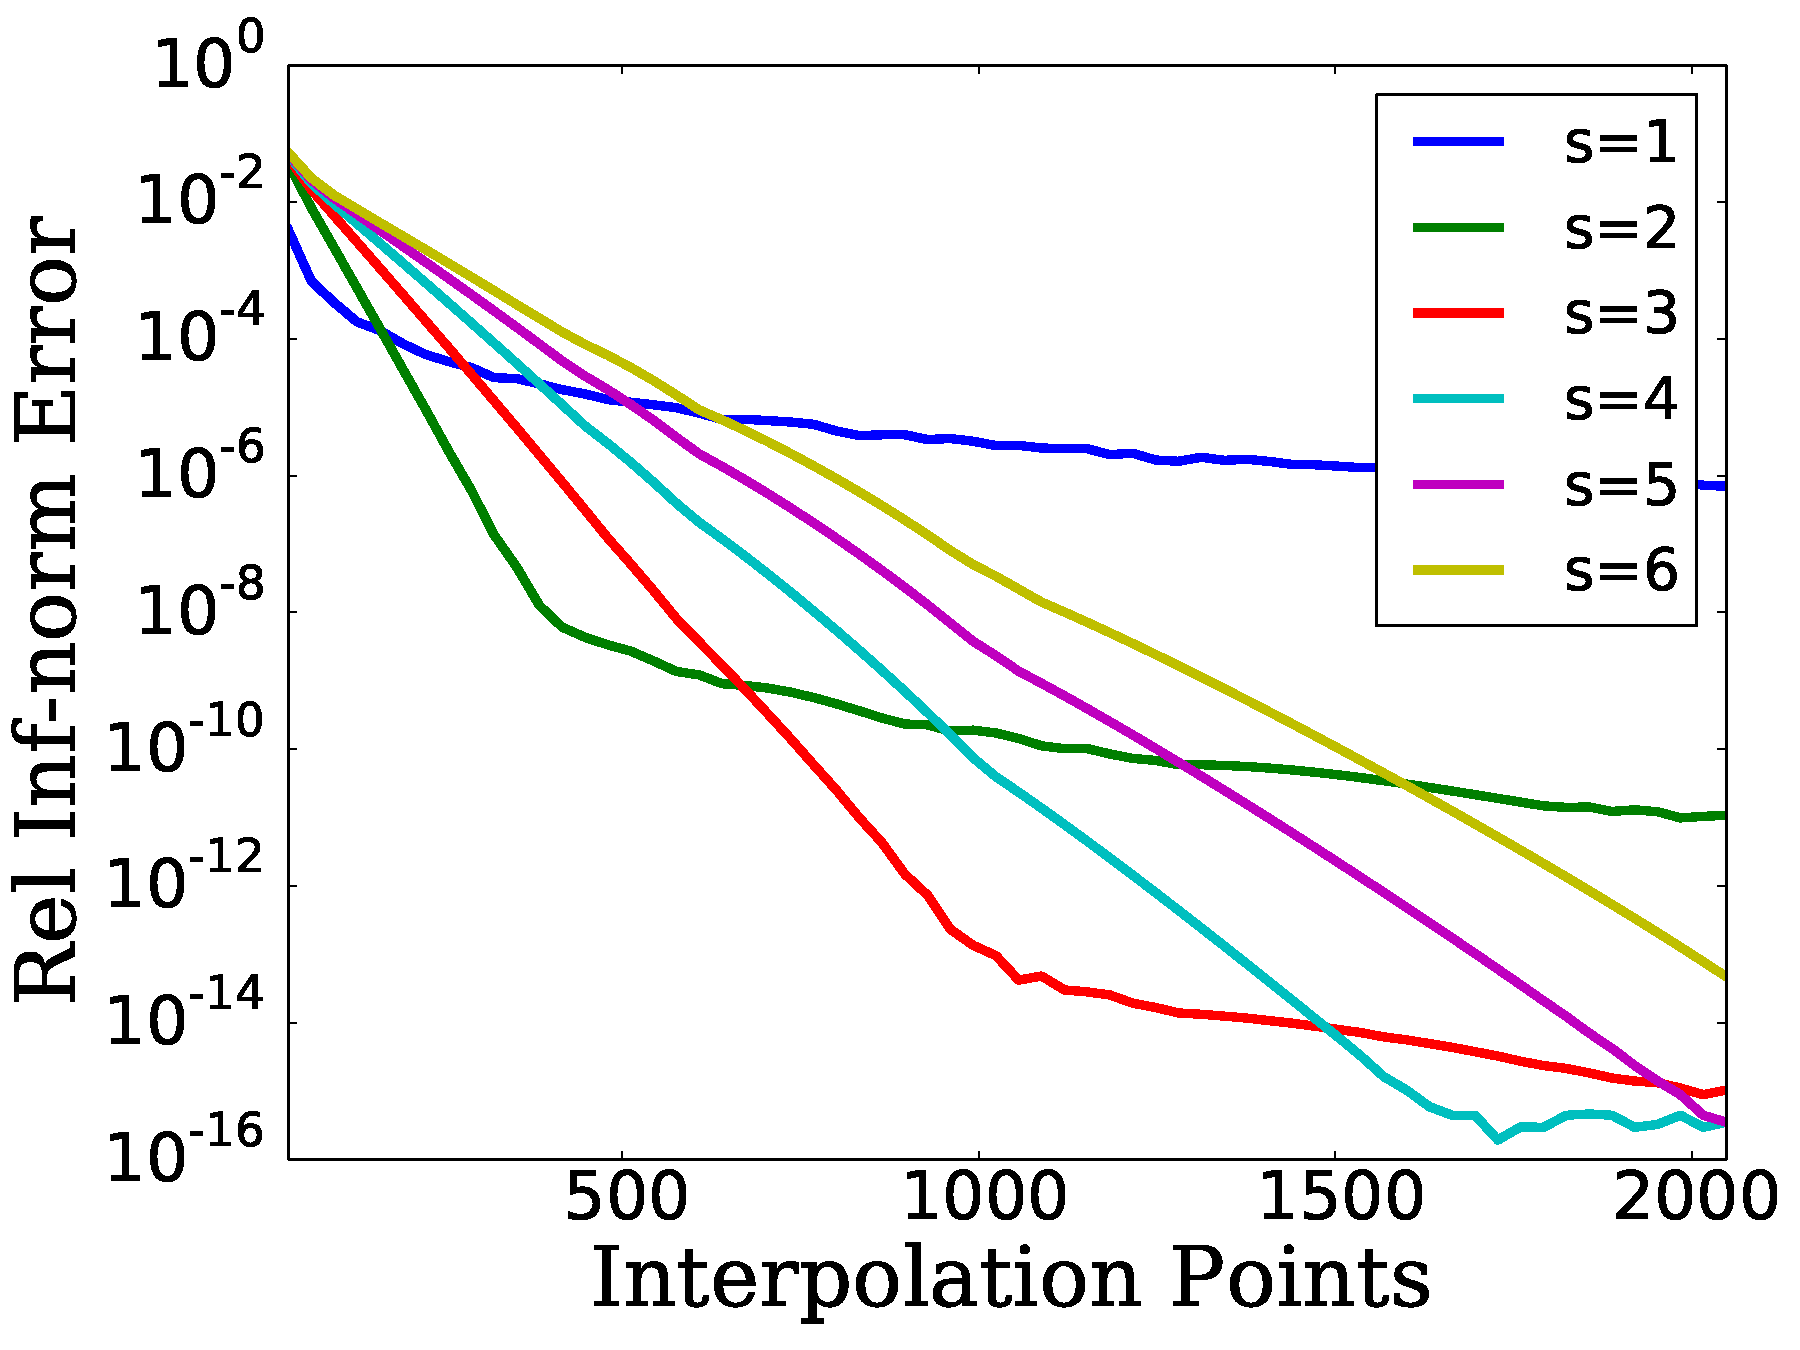
\includegraphics[width=\textwidth]{plots/msn_interp_fast_4n_rough_heaviside_2.pdf}
    \caption{Degree $4n$}
    \end{subfigure}

    \begin{subfigure}{0.45\textwidth}
    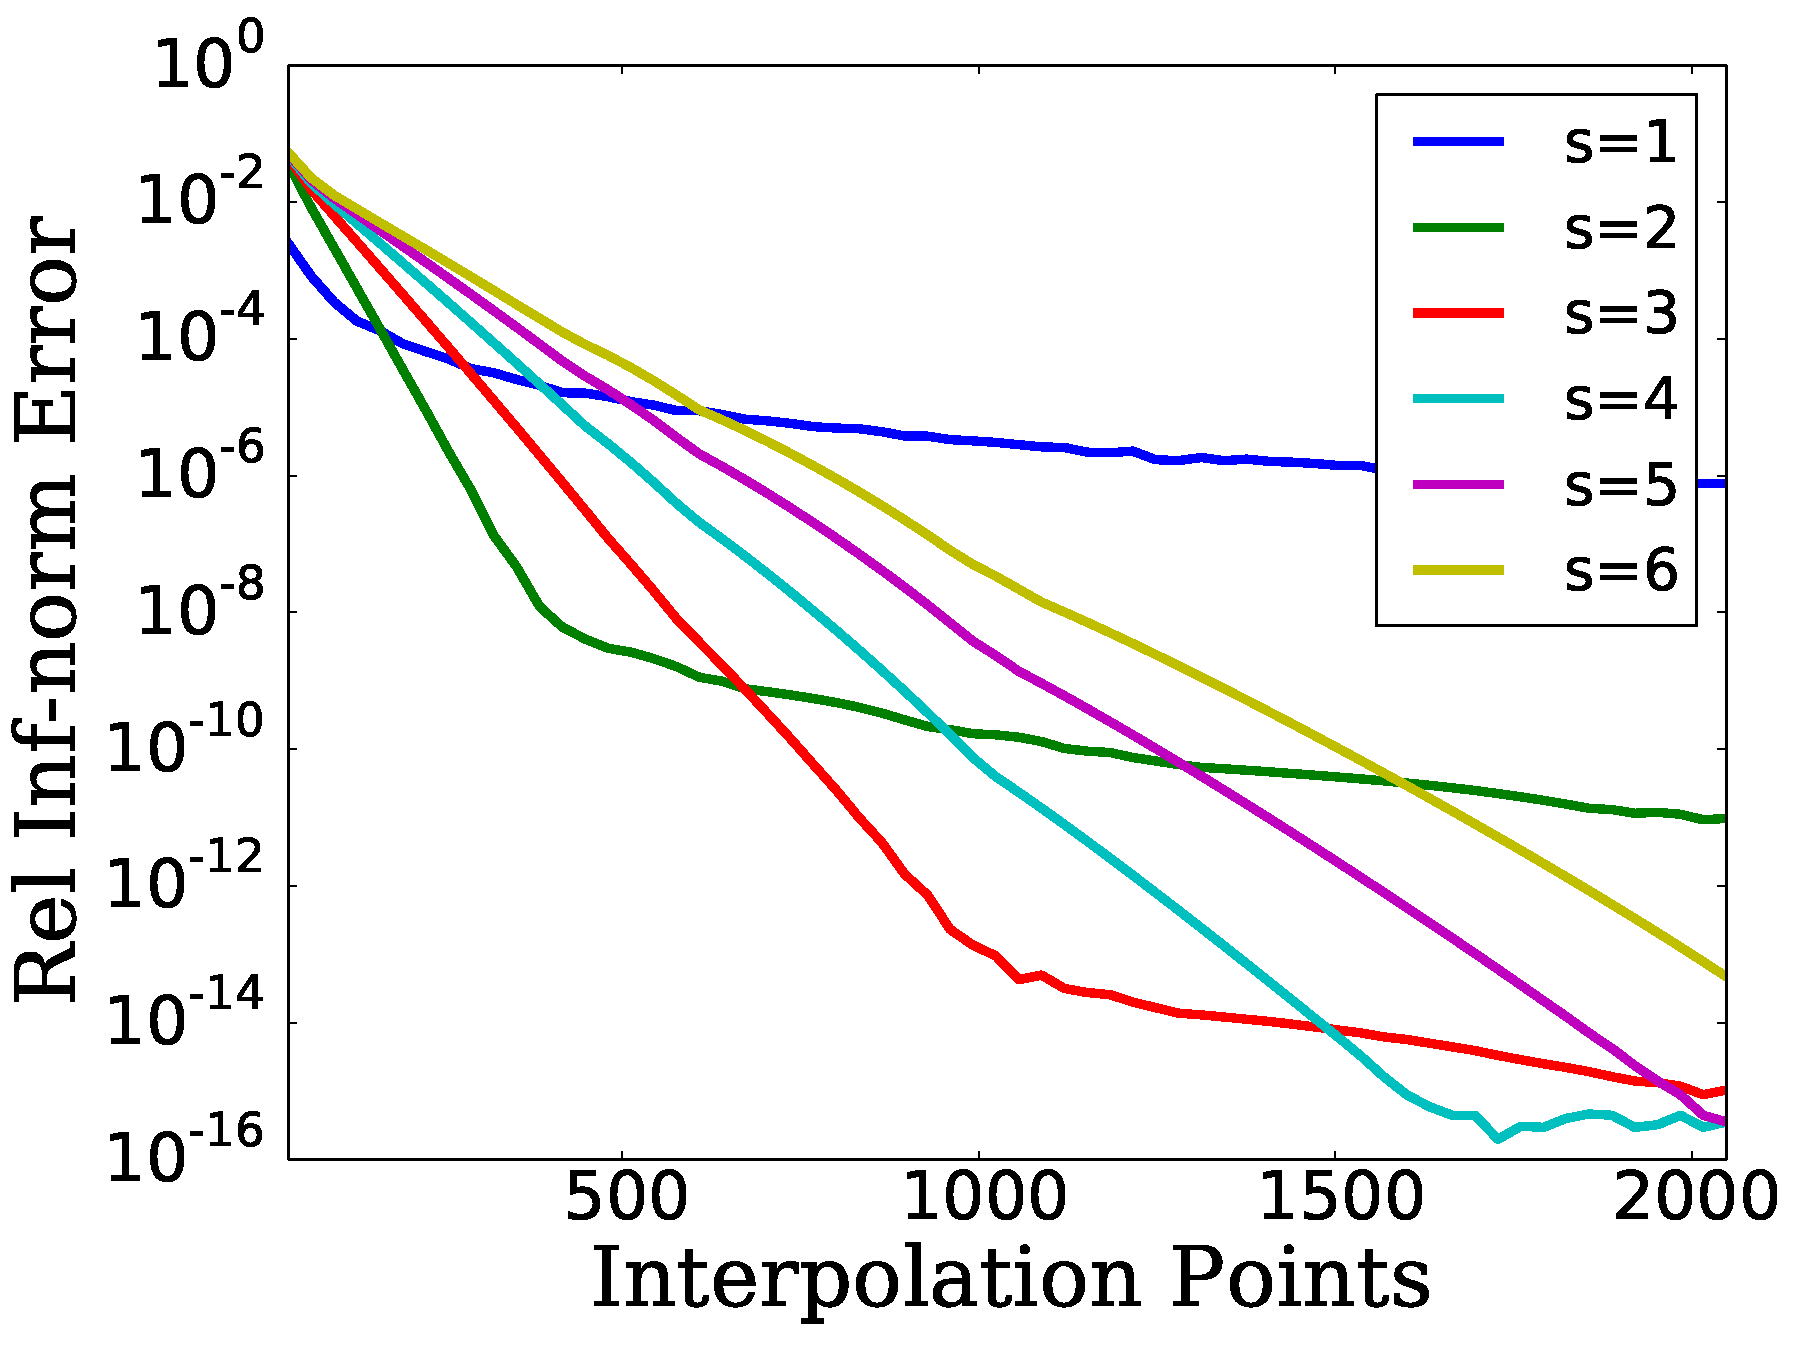
\includegraphics[width=\textwidth]{plots/msn_interp_fast_6n_rough_heaviside_2.pdf}
    \caption{Degree $6n$}
    \end{subfigure}
    \begin{subfigure}{0.45\textwidth}
    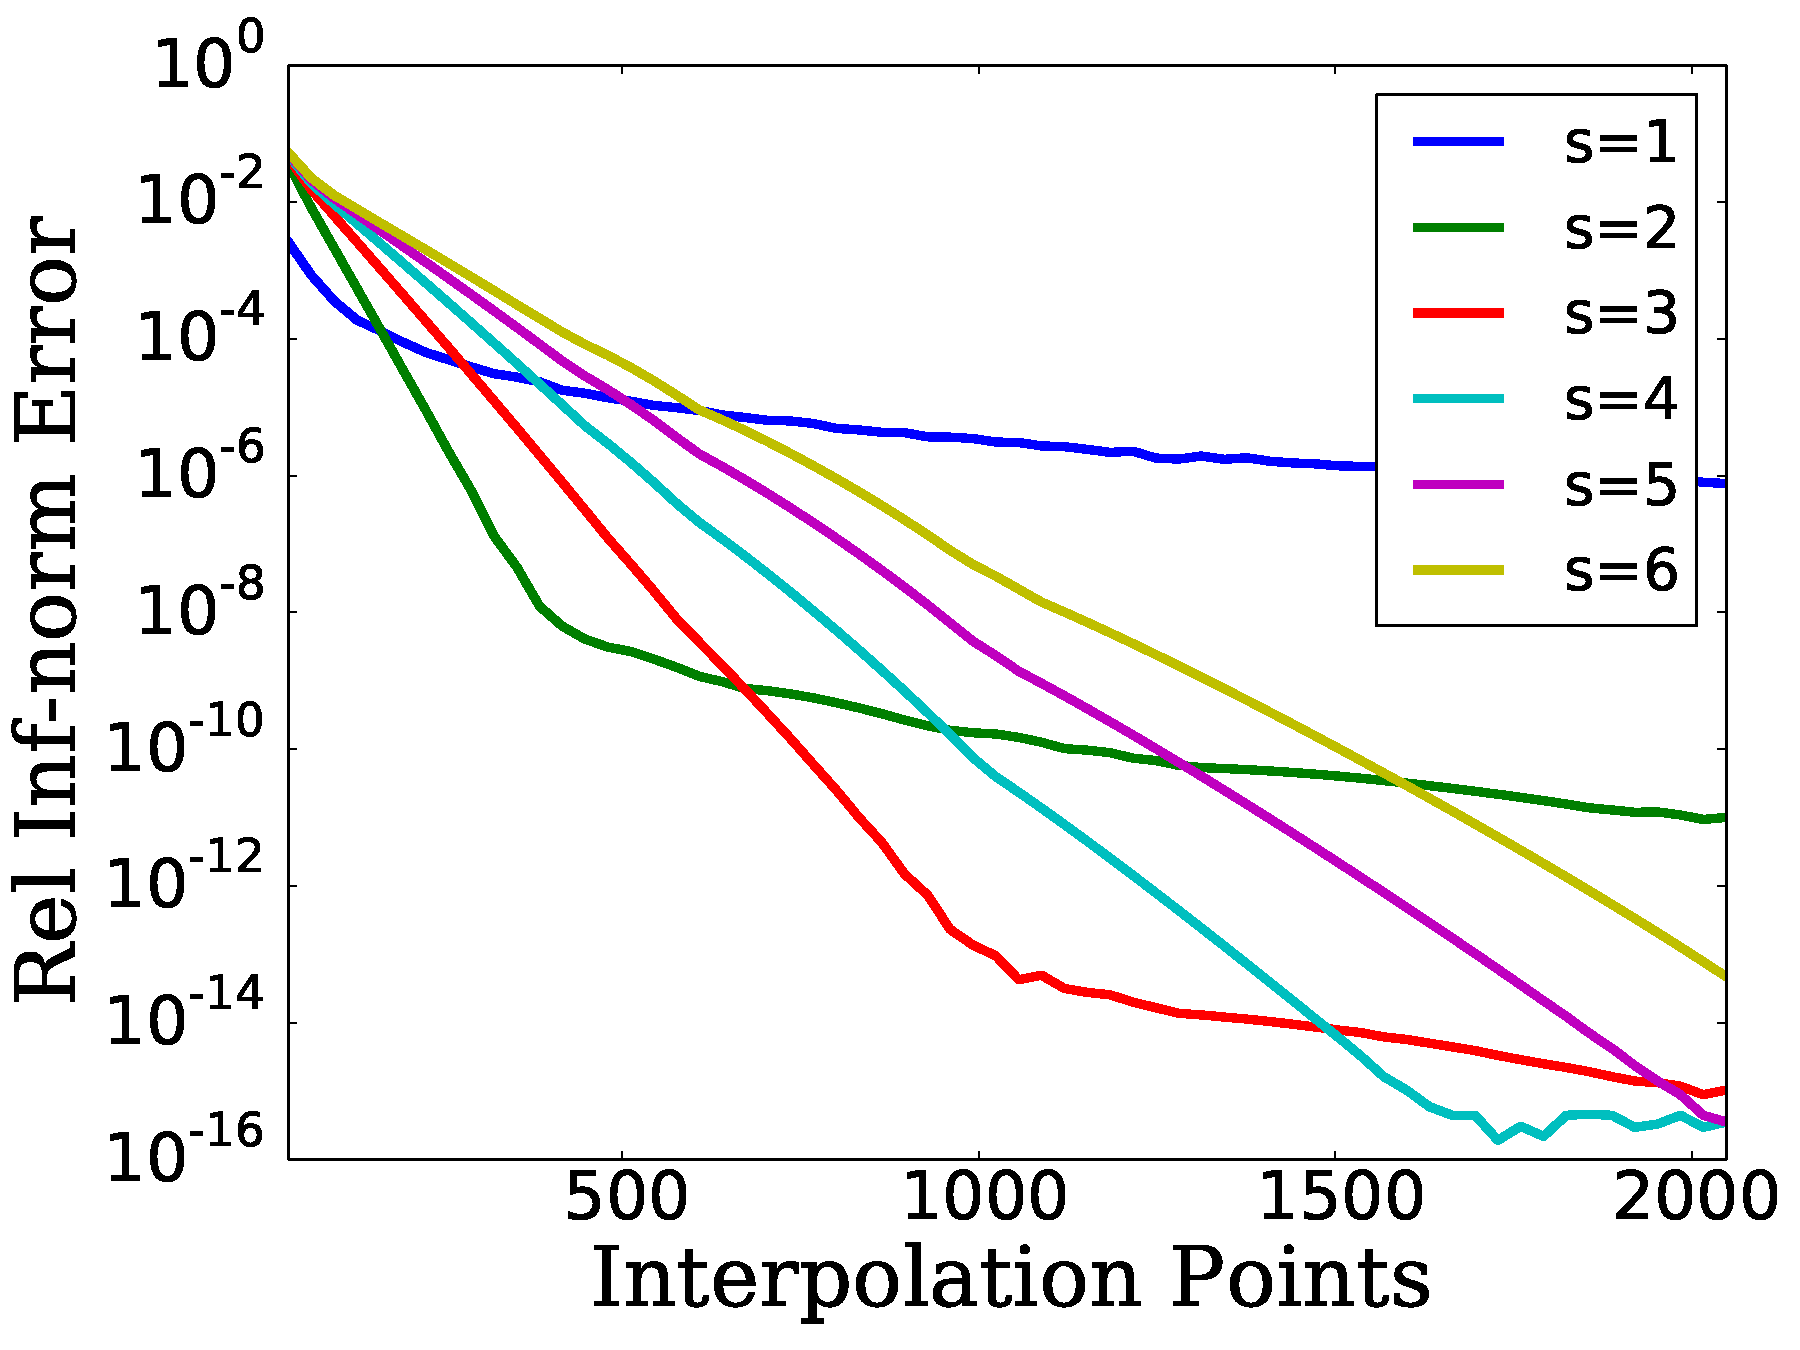
\includegraphics[width=\textwidth]{plots/msn_interp_fast_8n_rough_heaviside_2.pdf}
    \caption{Degree $8n$}
    \end{subfigure}
\caption[Example Plots of MSN Interpolation of Various Degrees]{
We show results for different interpolation degree.
For large $s$ values, there is no apparent advantage for using
a higher interpolation degree.
}
\label{fig:msn_comp_degree}
\end{figure}



